% LTeX: language=fr

\chapter{Réflexion sur les Procédures}










\section{Acquisition forensique}

L'acquisition forensique est divisée en trois parties: la préparation, l'acquisition des données en elle-même et la phase de post-acquisition. La préparation est se déroule à la fois longtemps avant de lancer l'acquisition forensique comme en installant les logiciels, mais aussi juste avant, en récupérant les identifiants du compte administrateur local de la machine, par exemple. Après avoir effectué l'acquisition, vient la phase de post-acquisition lors de laquelle, on va préparer ce qui vient ensuite: l'analyse des données forensiques.





\subsection{Préparation}

La \textit{préparation} commence longtemps avant l'acquisition des données forensiques. D'abord, au point de vue hardware, il faut obtenir des disques durs externes suffisamment grands pour pouvoir contenir les données des machines dont on veut faire l'analyse forensique. Il faut aussi qu'ils soient assez rapide pour essayer de gagner un maximum de temps lors de la copie des données sur le disque externe, c'est pour cela que la technologie SSD est recommandée, tout comme les dernières versions des connecteurs USB.

\begin{example}
    \hspace{0.45cm} Par exemple, pour un PC avec un disque dur de 256 Go et 8 Go de mémoire RAM, on pourrait penser qu'un disque dur externe de seulement 264 Go suffit. C'est cependant faux. La mémoire RAM qui sera acquise est plus grande que 8 Go à cause du swap, qui est le stockage d'une partie de la mémoire volatile sur le disque. De plus, il faut aussi suffisamment de place pour y mettre les outils dans le cas où la machine à analyser n'aurait qu'un seul port USB.
\end{example}

Un autre point qui est lié à la \textit{préparation} est l'isolement de la machine infectée du réseau. On peut facilement le faire avec Microsoft EDR (voir figure \ref{fig:microsoft-edr-isolate}). Le problème ne vient cependant pas toujours d'un malware qui aurait infecté le PC d'un utilisateur, mais il peut venir de l'utilisateur lui-même, par exemple parce qu'il aurait agi de manière répréhensible et voudrait en effacer les traces. Microsoft EDR ne permet pas de bloquer l'utilisateur pour l'empêcher d'accéder à son PC. 

\begin{figure}
    \centering
    \makebox[\textwidth]{
        \resizebox{9cm}{!}{
            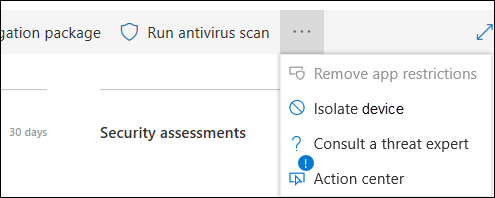
\includegraphics{images/incident-response/microsoft-edr-isolate.png}
        }
    }
    \caption{Isolation d'un appareil infecté dans Microsoft EDR pour empêcher l'infection de s'étendre dans le réseau.}
    \label{fig:microsoft-edr-isolate}
\end{figure}

Si on peut modifier à la fois l'AD et la machine de l'utilisateur, il y a bien moyen de le bloquer quand même. Pour l'empêcher d'effacer ses données à distance malgré tout, on devra:

\begin{enumerate}
    \item Désactiver l'utilisateur ou modifier son mot de passe dans l'AD pour empêcher l'utilisateur de se reconnecter à partir de l'AD.
    \item Supprimer le hash de son mot de passe stocké localement dans l'ordinateur pour empêcher l'utilisateur de se reconnecter localement.
    \item Déconnecter l'utilisateur à distance.
\end{enumerate}

Comme cela sortait un peu du cadre de mon TFE, je me suis arrêté après avoir testé que cette méthode fonctionnait bien mais je n'ai pas écrit de procédure complète sur son utilisation.

En bref, la phase de préparation consiste en la préparation matérielle et logicielle pour que l'acquisition forensique se passe au mieux au moment où en a besoin. De plus, dans les premiers instants de la réponse à incident, la préparation à l'acquisition forensique, en isolant les machines infectées et en obtenant les identifiants d'un compte administrateur local sur chacune des machines à analyser est essentiel pour ne pas perdre de temps lorsque l'analyste sera en leur possession.





\subsection{Mémoire volatile}

L'\textit{acquisition des données volatiles} doit se faire dès que l'analyste forensique a accès à la machine à analyser. D'ailleurs, selon le NIST, il faut décider à l'avance si on acquerra les données volatiles ou pas parce que le temps perdu à le décider fait qu'on risque de perdre des informations importantes. \cite{5} Au moins, la procédure pour les récupérer est plutôt simple puisqu'il suffit, après avoir brancher un disque dur externe contenant l'outil d'acquisition choisi, ici: Belkasoft RAM Capture, puis le lancer en tant qu'administrateur et choisir le lieu où la copie de la RAM doit être enregistré (voir figure \ref{fig:belkasoft-ram-capture}).

\begin{figure}
    \centering
    \makebox[\textwidth]{
        \resizebox{11cm}{!}{
            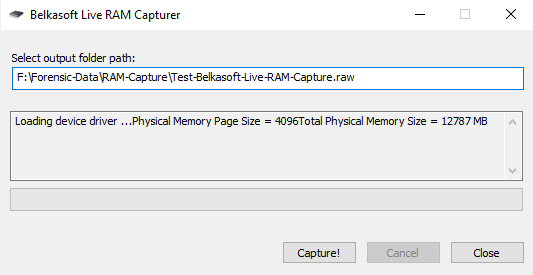
\includegraphics{images/RAM/ram-capture-01.png}
        }
    }
    \caption{Capture RAM avec Belkasoft RAM Capture.}
    \label{fig:belkasoft-ram-capture}
\end{figure}





\subsection{Mémoire de masse}

L'\textit{acquisition des données non-volatiles} est la troisième étape et se fait avec FTK Imager, qu'il faut bien sûr lancer avec des privilèges administrateur. C'est l'étape la plus longue, et sa vitesse dépend de deux facteurs: la rapidité en écriture sur le disque dur externe et de la vitesse de transfert qui dépend du type de transfert utilisé. Par exemple, un SSD utilisant un port USB 3.0 sera bien plus rapide qu'un simple disque dur utilisant la technologie USB 2.0.

Si le disque à analyser est chiffré avec BitLocker, il faut absolument récupérer la clé de chiffrement. Dans la plupart des organisations, elle sera enregistrée dans l'Active Directory. Si ce n'est pas le cas, on peut toujours la récupérer en ligne de commande avec: \texttt{manage-bde -protectors <lettre-de-lecteur> -get}. Cette commande doit être lancée avec des privilèges administrateurs, son utilisation est expliquée plus en détail dans la section sur les outils d'acquisition de données forensiques non-volatiles.





\subsection{Clé USB}

Lorsqu'on doit effectuer l'analyse forensique d'une clé USB, il faut, comme pour l'image disque, utiliser FTK Imager en tant qu'administrateur. Le problème de la clé USB est que dès qu'on la branche, on va commencer à modifier des données qui s'y trouvent parce que Windows va aller lire des données qui y sont présentes. Il y a deux solutions pour y remédier. La première est d'utiliser un élément hardware \textit{write-blocker} qui se place entre le port USB de l'ordinateur et la clé USB pour éviter de manière physique qu'on aille modifier des données. La seconde possibilité est de monter la clé USB en lecture seule en modifiant un paramètre Windows. Celui-ci se trouve dans le registre comme vous pouvez le voir sur la figure \ref{fig:usb-key-read-only} et il nécessite des droits administrateurs pour être modifié. \cite{12} Des tests ont été effectués dans le cadre du stage pour vérifier qu'une fois que ce changement est effectué, aucune modification quelle qu'elle soit ne sera apportée sur la clé USB.

\begin{figure}
    \centering
    \makebox[\textwidth]{
        \resizebox{19cm}{!}{
            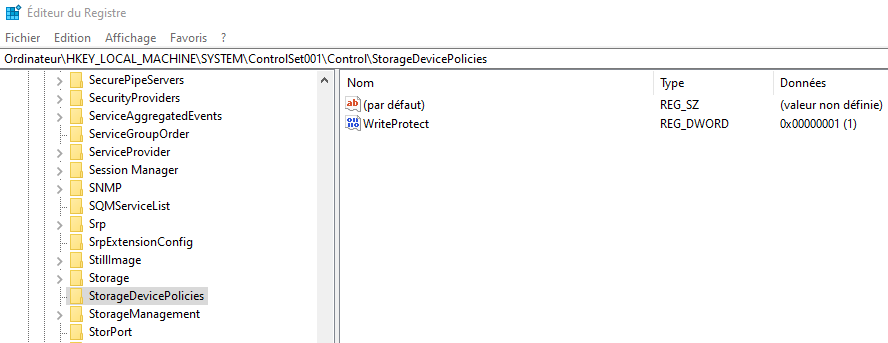
\includegraphics{images/Disque/read-only-registry.png}
        }
    }
    \caption{Modification d'une clé de registre pour monter une clé USB en lecture seule.}
    \label{fig:usb-key-read-only}
\end{figure}





\subsection{Post-acquisition}

La dernière étape est la \textit{post-acquisition}. Il s'agit de faire des copies pour pouvoir effectuer les analyses tout en cherchant à ne pas modifier les données. En plus de copier les données, on calcule aussi les hashs des données juste après l'acquisition pour montrer que les analystes n'ont pas modifié les données que ce soit volontairement ou par accident.










\section{Analyse de menaces}

\begin{figure}
    \centering
    \makebox[\textwidth]{
        \resizebox{16cm}{!}{
            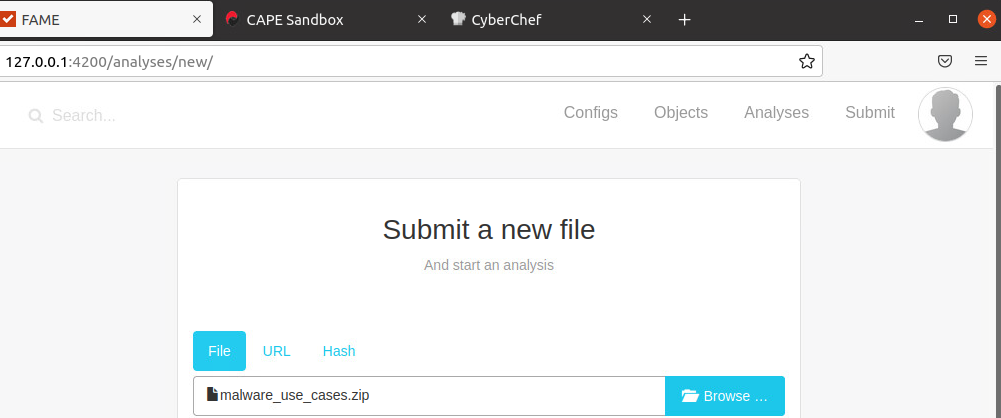
\includegraphics{images/malware/fame-submit.png}
        }
    }
    \caption{Interface de soumission de FAME.}
    \label{fig:fame-submission}
\end{figure}

La marche à suivre pour analyser un malware ou tout autre document supposé malicieux est simple grâce aux outils automatiques mis en place comme la plateforme d'analyse automatique de malwares FAME et la sandbox CAPE qui effectue des analyses dynamiques de malware dans une machine virtuelle imbriquée. Le seul souci est qu'il faut transférer le fichier à analyser depuis le PC de l'analyste vers la plateforme d'analyse qui se trouve dans un réseau isolé. Ceci a été expliqué plus en détail plus haut dans la section sur l'architecture de la solution. En résumé, il faut: se connecter en VPN au tenant NECS (NECS est le cloud NRB où est hébergée l'infrastructure), se connecter au serveur FTP pour y uploader le fichier à analyser, se connecter avec VMRC (VMWare Remote Console) à une machine d'analyse et télécharger le fichier en FTP depuis là pour lancer l'analyse via l'interface web (figure \ref{fig:fame-submission}).

L'analyse se fait de manière automatique. Par exemple, quand on soumet un mail qui a été signalé comme phishing par un utilisateur, une analyse de ses headers va être effectuée, les pièces jointes seront extraites et analysées à leur tour. On peut voir l'analyse des headers d'un de mes use cases sur la figure \ref{fig:fame-email-headers}. Grâce à cette analyse, on peut voir que le nom de domaine qui l'a envoyé est utilisé par un service de boîtes mails temporaires que l'on pourrait décider de bannir pour prévenir ce genre d'attaques à l'avenir.

\begin{figure}
    \centering
    \makebox[\textwidth]{
        \resizebox{19cm}{!}{
            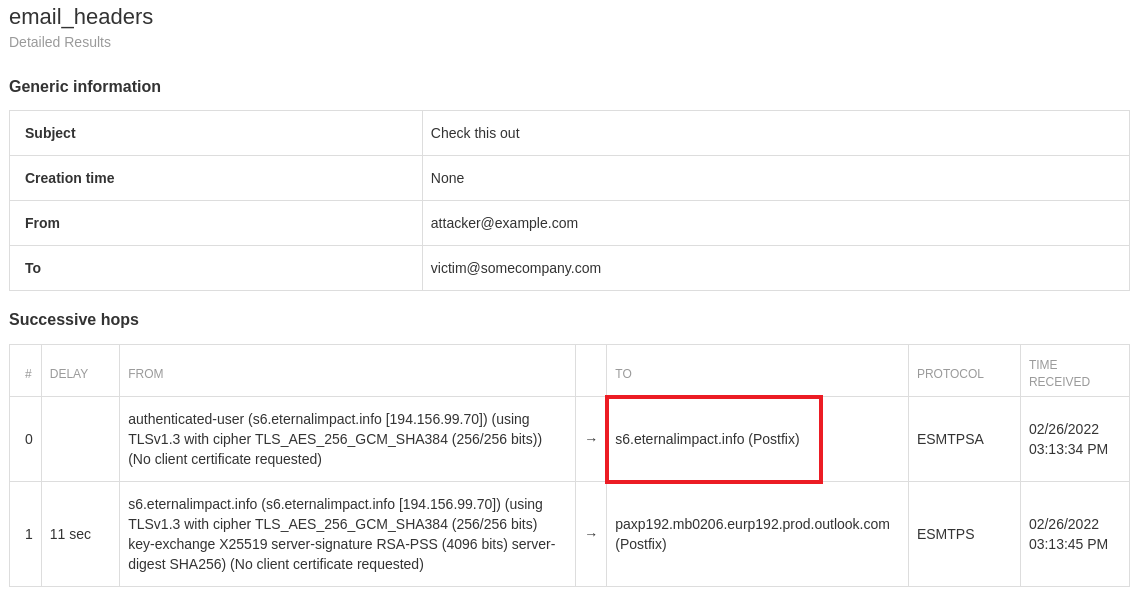
\includegraphics{images/malware/fame-analysis-11.png}
        }
    }
    \caption{Analyse des headers d'un email montrant que l'envoyeur est un service d'adresses email temporaires.}
    \label{fig:fame-email-headers}
\end{figure}

Dans le cas où les informations disponibles depuis l'interface de FAME en rapport avec l'analyse dynamique ne suffiraient pas, on peut toujours entrer plus dans le détail en cliquant sur \textit{View Report} comme sur la figure \ref{fig:fame-cape-report}. On arrive alors sur l'interface web de CAPE qu'on peut voir sur la figure \ref{fig:cape-analysis}.

\begin{figure}
    \centering
    \makebox[\textwidth]{
        \resizebox{17cm}{!}{
            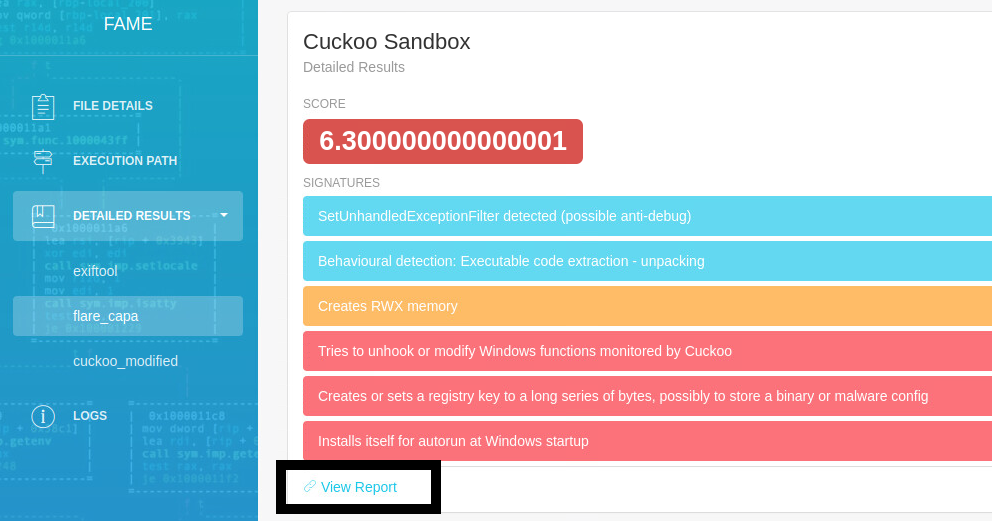
\includegraphics{images/malware/fame-analysis-09-report.png}
        }
    }
    \caption{Interface de résultats de FAME montrant les résultats des modules lancés, ici, CAPE Sandbox - dérivée de Cuckoo.}
    \label{fig:fame-cape-report}
\end{figure}

Sur l'interface web de CAPE, on peut voir les résultats de manière beaucoup plus précise et aussi en bien plus grande quantité. Par exemple, sur la figure \ref{fig:cape-analysis}, on peut voir non seulement que des tâches Windows ont été créées mais aussi lesquelles. On peut aussi y télécharger des fichiers. Il y a les fichiers qui ont été créés par le malware, un dump réseau qui contient tous les paquets qui ont transité sur le réseau en provenance et à destination de la sandbox, ainsi qu'un dump de la mémoire RAM de la machine virtuelle imbriquée infectée.

\begin{figure}
    \centering
    \makebox[\textwidth]{
        \resizebox{17cm}{!}{
            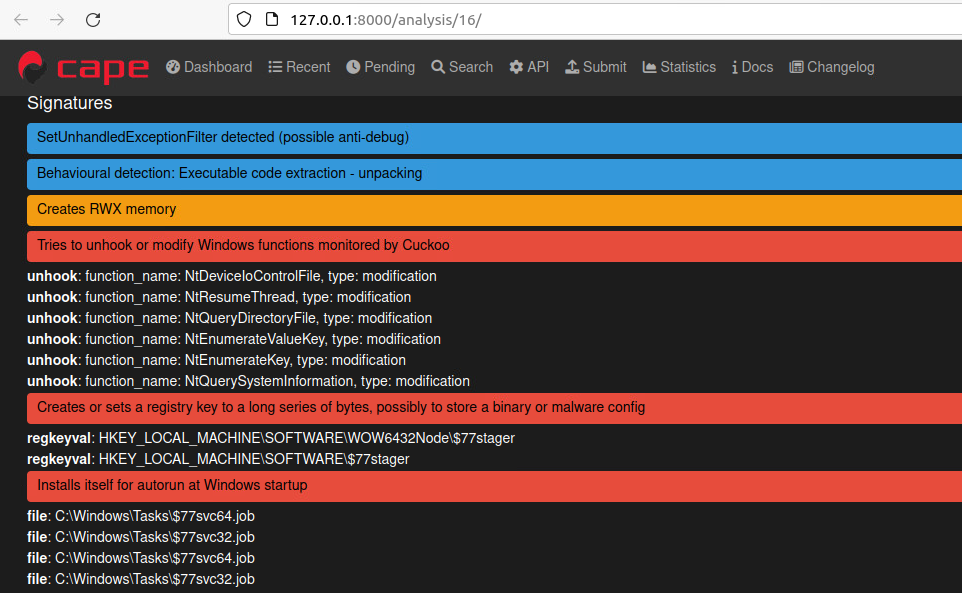
\includegraphics{images/malware/cape-analysis-02.png}
        }
    }
    \caption{Analyse du comportement du malware plus en détail avec CAPE Sandbox.}
    \label{fig:cape-analysis}
\end{figure}










\section{Analyse forensique}





\subsection{Extraire les données}

Pour analyser les informations présentes sur l'image d'un disque, il faut lancer plusieurs actions comme scanner les espaces vides du disque pour trouver des fichiers supprimés, copier les fichiers de grande importance forensique ou encore les parser pour normaliser l'information, ce qui rend l'analyse plus aisée. Mais la première chose à faire est de déchiffrer les données le cas échéant. Dans le cas d'un disque chiffré avec BitLocker, il faut monter l'image disque avec \textit{Arsenal Image Mounter} (figure \ref{fig:arsenal-image-mounter}). On peut ensuite la déchiffrer directement avec la clé dans l'explorateur de fichiers comme sur la figure \ref{fig:bitlocker}.

Après avoir monté l'image, on va en extraire les fichiers qui ont une importance forensique et normaliser les données de ces fichiers avec \textit{Kape}, un outil créé par l'entreprise Kroll. Il faut lancer le logiciel avec des privilèges administrateur pour qu'il puisse lire les fichiers systèmes. Vous pouvez voir l'interface graphique de Kape appelée \textit{gkape} (figure \ref{fig:gkape}). Elle est divisée en deux parties:

\begin{itemize}
    \item La partie \textit{Target} sert à configurer les extractions de fichiers de l'image montée pour en placer des copies dans un dossier. Quelques exemples de fichiers sont les logs, les registres, la MFT (Master File Table, l'index principal du système de fichiers NTFS, utilisé par Windows), etc.
    \item La partie \textit{Module} sert à configurer le parsing des données extraites, par exemple en transformant les logs au format CSV et en les regroupant sous un seul fichier ou en transposant les données stockées dans la MFT au format CSV.
\end{itemize}

\begin{figure}
    \centering
    \makebox[\textwidth]{
        \resizebox{19cm}{!}{
            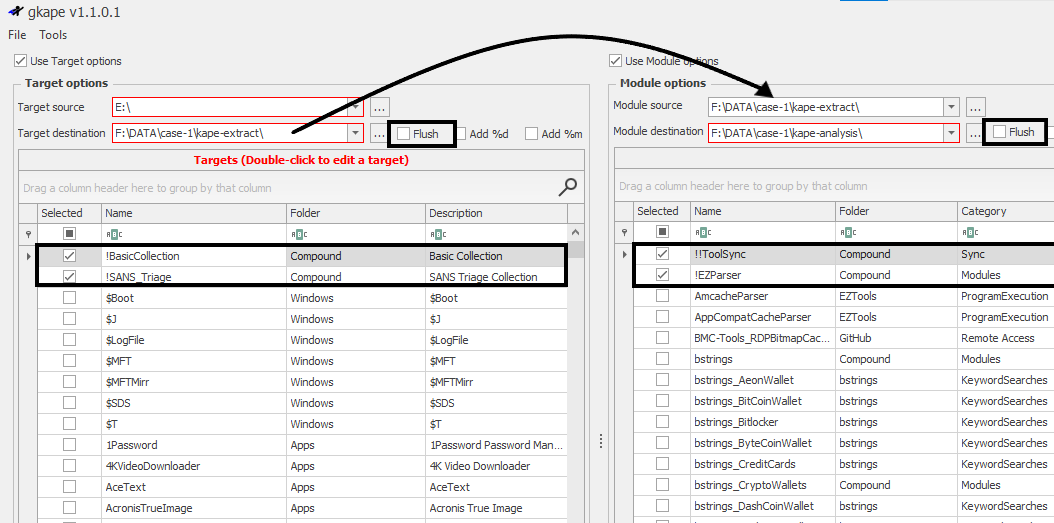
\includegraphics{images/Disque/kape-03.png}
        }
    }
    \caption{Interface graphique de Kape: \textit{gkape}.}
    \label{fig:gkape}
\end{figure}


\textit{Autopsy} est un logiciel d'analyse disque qui va nous permettre d'analyser les espaces vides de l'image disque pour voir s'il n'y a pas de fichiers supprimés qui s'y trouveraient. Il faut lancer ce programme avec des privilèges administrateur si l'image a été montée, mais si on analyse le fichier qui est l'image disque, on n'en a pas besoin (ça dépend donc de si le disque est chiffré ou non). En plus de cela, Autopsy possède une série de modules qui vont aller scanner les fichiers pour en extraire de l'information intéressante (voir figure \ref{fig:autopsy-ingest}). Les modules les plus intéressants sont:

\begin{itemize}
    \item \textit{Recent Activity}: il recherche les documents récents, les programmes installés, les données du navigateur comme les comptes enregistrés, l'historique de navigation et les favoris.
    \item \textit{File Type Identification}: il identifie le type des fichiers en fonction de leur signature.
    \item \textit{Extension Mismatch Detector}: il liste les documents dont l'extension ne correspond pas à leur type. Par exemple, un exécutable avec une extension \textit{.txt} se ferait détecter par ce module.
    \item \textit{Email Parser}: il liste les emails enregistrés localement sur l'ordinateur.
    \item \textit{Encryption Detection}: il va chercher les fichiers qui ont une entropie élevée, ce qui est indicateur d'un chiffrement.
    \item \textit{Interesting File Identifier}: ce module aurait peut-être dû être nommé \textit{Interesting Programs Identifier} parce qu'il va chercher les programmes intéressants comme les logiciels de chiffrement, les VPN, les crypto wallets, etc.
\end{itemize}

Les modules \textit{Embedded File Extractor} et \textit{Virtual Machine Extractor} peuvent être très utiles mais ils peuvent prendre énormément de temps. Ce n'est donc pas à activer en toutes circonstances.

\begin{figure}
    \centering
    \makebox[\textwidth]{
        \resizebox{17cm}{!}{
            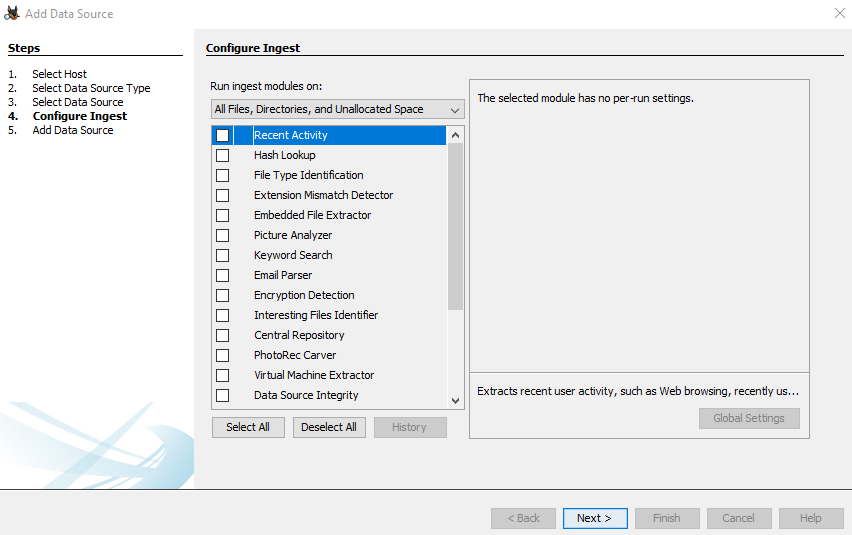
\includegraphics{images/Disque/autopsy-07.png}
        }
    }
    \caption{Ensemble de modules d'Autopsy qui peuvent être lancés pour analyser une image disque.}
    \label{fig:autopsy-ingest}
\end{figure}


\textit{Thor Lite} est un scanner anti-virus qu'il faut lancer en tant qu'administrateur. Ses résultats sont faciles à analyser. On peut le lancer avec la commande suivante: \texttt{.$\backslash$thor64-lite.exe -{}-intense -a FileSystem -{}-path E:$\backslash$ -o .$\backslash$output$\backslash$}





\subsection{Analyse des données}



\subsubsection{Analyse de logs}

\textit{Chainsaw} est un outil d'analyse de logs Windows (au format evtx) qui liste les évènements suspicieux, et en particulier, tout ce qui est lié au mouvement latéral. La première chose à faire avant de l'utiliser est de trouver le dossier contenant les logs extraits par Kape. Les logs sont normalement stockés dans le dossier \texttt{C:$\backslash$Windows$\backslash$System32$\backslash$winevt$\backslash$logs$\backslash$}. Si on les a extraits avec Kape et pas manuellement, ils devraient se trouver dans un dossier comme \\
\texttt{E:$\backslash$DATA$\backslash$case-1$\backslash$kape-extract$\backslash$F$\backslash$Windows$\backslash$System32$\backslash$winevt$\backslash$logs$\backslash$} \\
Ensuite, on peut lancer chainsaw avec peu de règles pour commencer, afin d'avoir une première vue sur les données. On pourra ensuite l'utiliser avec plus de règles pour avoir une vue complète et obtenir toutes les alertes. On peut le faire avec les commandes suivantes:

\begin{enumerate}
    \item Vue d'ensemble: \texttt{.$\backslash$chainsaw.exe hunt <dossier-logs> -{}- lateral-all}
    \item Appliquer toutes les règles: \\
    \texttt{.$\backslash$chainsaw.exe hunt <dossier-logs> -{}- lateral-all \\
    -{}-rules .$\backslash$sigma\_rules$\backslash$ \\
    -{}-mapping .$\backslash$mapping\_files$\backslash$sigma-mapping.yml}
\end{enumerate}

Sur la figure \ref{fig:chainsaw-lateral-movement}, on peut voir que chainsaw a récupéré toutes les connexions à distances effectuées sur la machines. Ces évènements peuvent être indicateurs de mouvement latéral vers la machine.

\begin{example}
    \hspace{0.45cm} Par exemple, un attaquant pourrait avoir créé une tâche à distance sur la machine pour l'infecter, ce qui aurait généré à la fois un log de connexion à distance et un log de création de tâche. En analysant les évènements autour de ces connexions réseau, on peut trouver des traces de mouvement latéral, ce qui peut conduire à une escalade dans la réponse à incident.
\end{example}

\begin{figure}
    \centering
    \makebox[\textwidth]{
        \resizebox{16cm}{!}{
            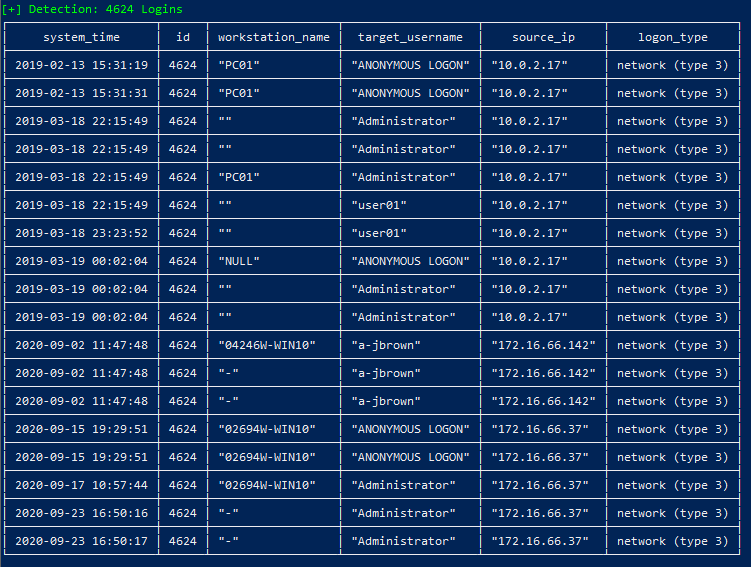
\includegraphics{images/Disque/chainsaw-02.png}
        }
    }
    \caption{Analyse des connexions à distance indiquant des possibles mouvements latéraux avec chainsaw.}
    \label{fig:chainsaw-lateral-movement}
\end{figure}



\subsubsection{Analyse des fichiers intéressants d'un point de vue forensique}

Les outils pour analyser les fichiers intéressants d'un point de vue forensique ont été créés par Erik Zimmerman, qui travaille chez Kroll, l'entreprise qui a créé Kape. Les trois plus intéressants sont \textit{Registry Explorer} et \textit{Timeline Explorer}, mais je vais présenter aussi \textit{Shellbags Explorer} dans cette section.

\textit{Registry Explorer} permet de lire les clés de registres et même de les corriger avec les logs si elles sont \textit{sales} (comme une base de données corrompue qu'on peut nettoyer grâce aux logs). C'est très utile de pouvoir naviguer dans le registre pour y retrouver des données. Par exemple, sur la figure \ref{fig:zimmerman-registry-explorer}, on peut voir la date à laquelle une clé USB a été branchée pour la première fois. Dans le cas où un PC a été infecté par une clé USB, ça peut aider à trouver la date d'infection.

\begin{figure}
    \centering
    \makebox[\textwidth]{
        \resizebox{19cm}{!}{
            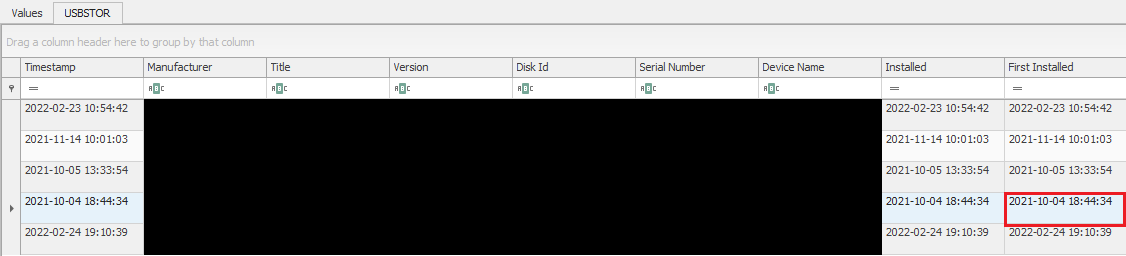
\includegraphics{images/Disque/zimmerman-02.png}
        }
    }
    \caption{Analyse des registres avec Registry Explorer pour trouver quand une clé USB a été branchée pour la première fois.}
    \label{fig:zimmerman-registry-explorer}
\end{figure}

\textit{Timeline Explorer}, c'est un peu un substitut à Excel que l'on peut utiliser pour analyser les fichiers CSV générés par Kape. Bien qu'il ait beaucoup moins de fonctionnalités qu'Excel, il peut analyser des fichiers beaucoup plus gros aisément et ne requiert pas de licence. On peut, par exemple, analyser les données de la MFT, des registres ou encore des preuves d'exécution de programmes compilées par Kape. Sur la figure \ref{fig:zimmerman-timeline-explorer}, vous pouvez voir l'analyse de la MFT d'un PC infecté par un malware qui a modifié la date de création \textit{Created0x10} de ses fichiers pour faire croire qu'ils avaient étés créés en 2019 ou lieu de 2022. Ce timestamp est accessible via l'API Win32 mais la MFT utilise un deuxième timestamp pour la création des fichiers: le \textit{Created0x30}, qui n'est accessible que par le kernel Windows et n'a donc pas été modifié par le malware.

\begin{figure}
    \centering
    \makebox[\textwidth]{
        \resizebox{18cm}{!}{
            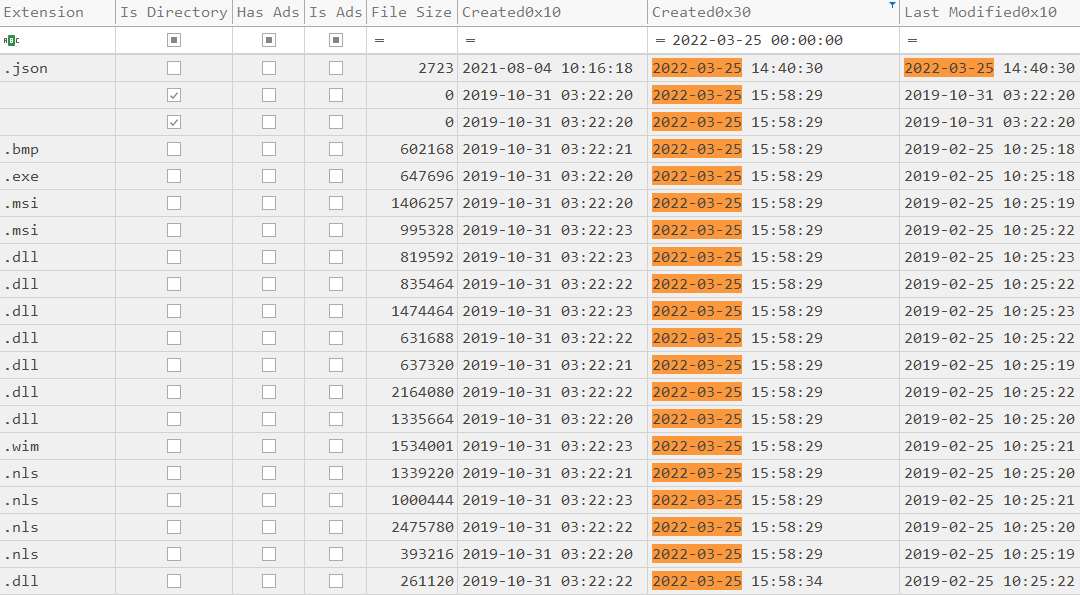
\includegraphics{images/Disque/zimmerman-03.png}
        }
    }
    \caption{Analyse de la MFT avec Timeline Explorer pour trouver les fichiers créés à certaine date malgré que le timestamp ait été modifié.}
    \label{fig:zimmerman-timeline-explorer}
\end{figure}

Quand on visite un dossier avec l'explorateur de fichiers de Windows, on peut modifier l'affichage des fichiers qu'il contient pour les trier en fonction de la date, de l'ordre alphabétique ou encore changer l'affichage pour montrer une miniature des images. Ces paramètres sont enregistrés par Windows pour améliorer l'expérience utilisateur mais permettent aussi à un enquêteur forensique de trouver la preuve qu'un dossier a bel et bien existé et a été visité par un utilisateur.

\textit{Shellbags Explorer} permet, comme son nom l'indique, d'analyser les shellbags. Sur la figure \ref{fig:zimmerman-shellbags-explorer}, vous pouvez voir les dossier consulté par un utilisateur, y compris sur un serveur FTP. En utilisant ces informations, on peut prouver l'existence de serveurs de fichiers personnels et l'existence de dossiers potentiellements sensibles sur ceux-ci.

\begin{figure}
    \centering
    \makebox[\textwidth]{
        \resizebox{19cm}{!}{
            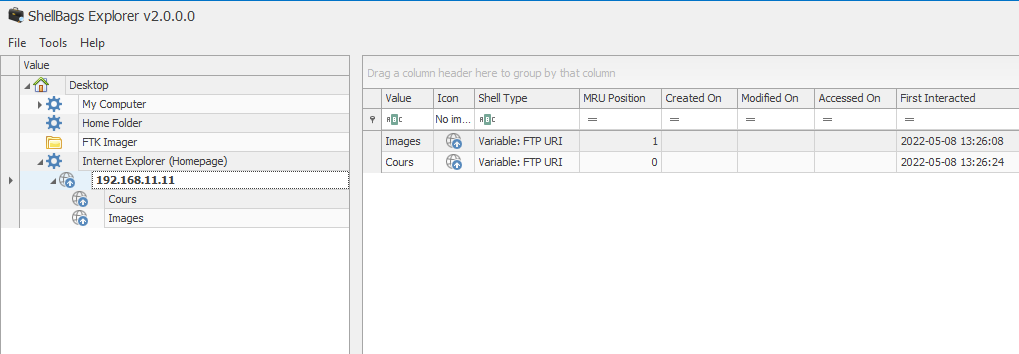
\includegraphics{images/Disque/zimmerman-01.png}
        }
    }
    \caption{Analyse des shellbags avec Shellbags Explorer pour chercher des traces d'exfiltration de données.}
    \label{fig:zimmerman-shellbags-explorer}
\end{figure}

Il faut faire attention aux différence de zones horaires et au changement d'heure. Par exemple, lorsqu'on analyse un système compromis avant le changement d'heure, on aura deux types de données. Premièrement, il y a celles qui sont indépendantes de la configuration de la machine d'analyse, c'est généralement parce que la date et l'heure de l'évènement est stockée directement. Deuxièmement, il y a celles qui ont un timestamp dépendant de la configuration de la machine, comme lorsqu'on utilise \textit{Unix epoch} qui compte le nombre de secondes depuis le 1er janvier 1970 à minuit UTC. Dans ce cas, la date affichée à l'analyste sera dépendante de la zone horaire de sa machine d'analyse puisque la zone horaire de la machine analysée n'est pas contenue dans la donnée.



\subsubsection{Analyse générale du disque}

Avec \textit{Autopsy}, on peut voir la structure du système de fichiers. Cela peut servir pour lire certains fichiers, par exemple, en allant lire le fichier contenant l'historique des commandes powershell. Grâce à l'analyse des fichiers supprimés, on peut aussi retrouver des données qu'un utilisateur a peut-être voulu cacher. Et en cherchant à travers l'historique des documents récents, plutôt que de devoir analyser l'ensemble des documents, il est possible de choisir, une poignée de documents récents à analyser si on suspecte ce vecteur d'infection d'avoir compromis un système. De manière générale, l'enquête sur Autopsy va se faire sur ses données qui ont été rassemblées sous la section \textit{Data Artifacts} que vous pouvez voir sur la figure \ref{fig:autopsy-analysis} qui regroupe un ensemble de données intéressantes.

\begin{figure}
    \centering
    \makebox[\textwidth]{
        \resizebox{16cm}{!}{
            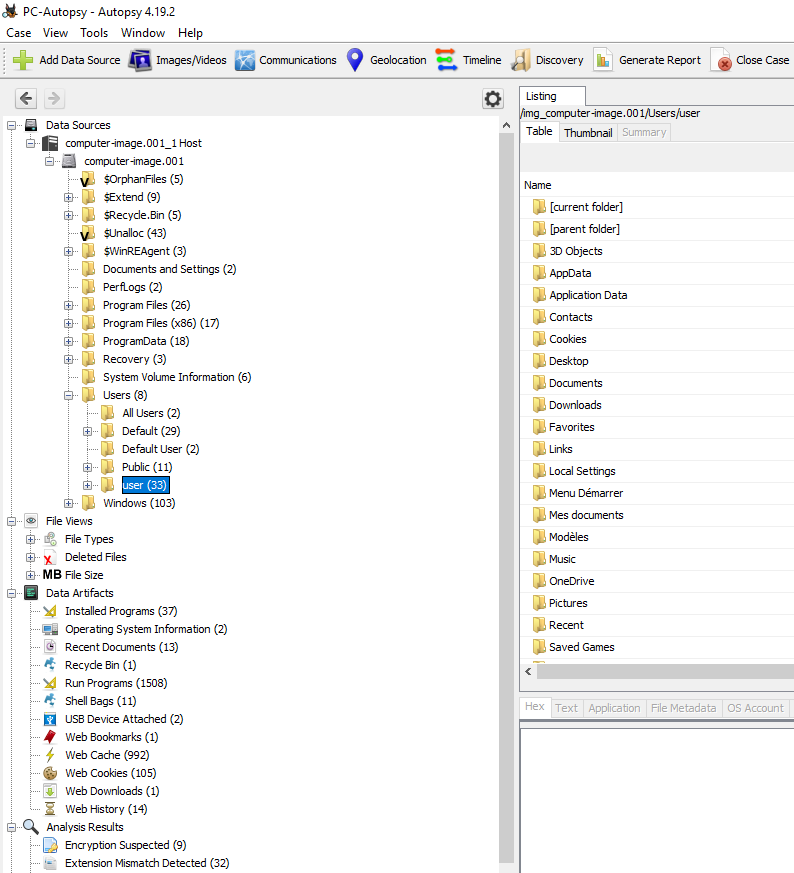
\includegraphics{images/Disque/autopsy-11.png}
        }
    }
    \caption{Analyse d'une image disque avec Autopsy.}
    \label{fig:autopsy-analysis}
\end{figure}





\subsection{Analyse de la mémoire volatile}

L'outil d'analyse de la mémoire volatile utilisé ici est Volatility 2 qui est un framework open source utilisé en ligne de commande en précisant un module. Il existe un ensemble de modules existant, à la fois supportés par le framework et d'autres écrits par la communauté. Un autre point important à soulever est que la mémoire RAM est différente en fonction de la machine dont elle provient. Pour pouvoir analyser un dump mémoire, il faut donc utiliser un profil qui correspond à la machine analysée, par exemple: Windows 10 x64 ou Windows 7 x86. La structure d'une commande dans Volatility contient donc ces deux éléments, le profil et le module en option: \texttt{volatility -f <dump-mémoire> -{}-profile=<trouvé-avec-imageinfo> <module>}

\begin{figure}
    \centering
    \makebox[\textwidth]{
        \resizebox{13cm}{!}{
            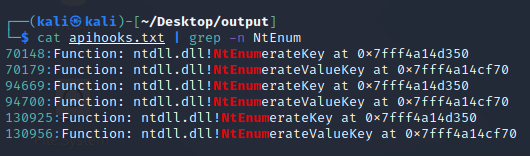
\includegraphics{images/RAM/volatility-rootkit-hooked-functions.png}
        }
    }
    \caption{Fonctions hookées par un rootkit listées avec Volatility.}
    \label{fig:volatility-rootkit}
\end{figure}

La méthode pour analyser un dump mémoire est donc la suivante: \cite{13}

\begin{enumerate}
    \item Identifier le profil de l'image avec: \textit{imageinfo} (à lancer sans l'option \textit{profile}).
    \item Identifier les processus malveillants:
    \begin{itemize}
        \item Lister les processus cachés: processus listés par \texttt{psscan}, mais pas par \texttt{pslist}. La comparaison est facile avec \texttt{psxview} qui affiche un tableau de comparaison.
        \item Chercher un processus "système" qui a un parent anormal: \texttt{pstree}.
        \item Identifier un processus injecté avec la méthode de process hollowing: \texttt{hollowfind}.
        \item Lister les pages mémoires suspectes avec des permissions en écriture et exécution, ce qui permet d'écrire et exécuter du code dans un autre processus par exemple: \texttt{malfind}.
    \end{itemize}
    \item Analyser les artefacts réseau: \textit{netscan}, par exemple l'utilisation du port 4444 est suspecte car c'est le port configuré par défaut par l'outil metasploit.
    \item Chercher la présence d'un rootkit en cherchant des fonctions Windows qui ont été modifiées pour cacher le rootkit:
    \begin{itemize}
        \item Liste des hooks sur les fonctions de l'API Windows: \texttt{apihooks}, vous pouvez voir un exemple sur la figure \ref{fig:volatility-rootkit} que des fonctions servant à lister les clés de registres ont été modifiées par un rootkit pour cacher certaines clés.
        \item Liste des hooks dans le System Service Descriptor Table (la table d'adressage des API): \texttt{ssdt} (exemple de hooks importants: \texttt{<volatility-ssdt> | egrep -v '(ntoskrnl|win32k)'})
    \end{itemize}
    \item Autres données intéressantes à analyser:
    \begin{itemize}
        \item Afficher l'historique des commandes: \textit{cmdscan}, ce n'est pas stocké sur le disque, c'est donc la seule manière de l'obtenir.
        \item Lister des clés intéressantes dans les registres: \textit{autoruns} et \textit{userassist}, vous pouvez voir un exemple sur la figure \ref{fig:volatility-userassist} où on voit la preuve que l'exécutable \textit{Install.exe} a été exécuté.
        \item Liste des services: \textit{svcscan}.
        \item Extraire un processus, une librairie ou un driver: \textit{procdump}, \textit{dlldump}, \textit{moddump}.
    \end{itemize}
\end{enumerate}

\begin{figure}
    \centering
    \makebox[\textwidth]{
        \resizebox{16cm}{!}{
            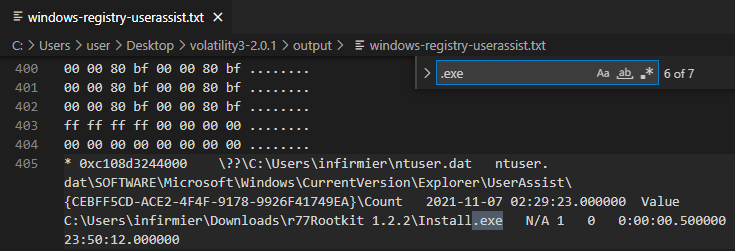
\includegraphics{images/RAM/volatility-userassist-executed-programs.png}
        }
    }
    \caption{Preuves de l'exécution d'un exécutable grâce à une clé userassist dans le registre listée avec Volatility.}
    \label{fig:volatility-userassist}
\end{figure}

